\begin{prp}[count=7] Soit une fonction affine $f\colon x\mapsto ax+b$.
\begin{itemize}
\item Si $a<0$ alors $f$ est (strictement) \textcolor{red}{décroissante}: \hfill
\begin{minipage}[c]{0.45\linewidth}
\begin{tikzpicture}
\tikzset{arrow style/.style={red,%
					line width=0.75pt,->,%
					>= latex',%
					shorten >= 6pt,%
					shorten <= 6pt}}
\tkzTabInit[lgt=1.5,espcl=3]%,deltacl=0.4
{$x$/0.5,$f(x)$/0.9}{$-\infty$,$+\infty$}%
\tkzTabVar{+/ ,-/ }%
\end{tikzpicture}
\end{minipage}
\item Si $a>0$ alors $f$ est (strictement)  \textcolor{red}{croissante} : \hfill
\begin{minipage}[c]{0.45\linewidth}
\begin{tikzpicture}
\tikzset{arrow style/.style={red,%
					line width=0.75pt,->,%
					>= latex',%
					shorten >= 6pt,%
					shorten <= 6pt}}
\tkzTabInit[lgt=1.5,espcl=3]%,deltacl=0.4
{$x$/0.5,$f(x)$/0.9}{$-\infty$,$+\infty$}%
\tkzTabVar{-/ ,+/ }%
\end{tikzpicture}
\end{minipage}
\item Si $a=0$ alors $f$ est \textcolor{red}{constante}: \hfill
\begin{minipage}[c]{0.45\linewidth}
\begin{tikzpicture}
\tikzset{arrow style/.style={red,%
					line width=0.75pt,->,%
					>= latex',%
					shorten >= 6pt,%
					shorten <= 6pt}}
\tkzTabInit[lgt=1.5,espcl=3]%,deltacl=0.4
{$x$/0.5,$f(x)$/0.9}{$-\infty$,$+\infty$}%
%\tkzTabVar{+/ ,+/ }%
\draw[arrow style] ($(N11)!0.5!(N12)$)--($(N21)!0.5!(N22)$);
\end{tikzpicture}
\end{minipage}
\end{itemize}
\end{prp}
